% Flat full-width framework. Abstract runs (no numbers), layered merge,
% a side cost model that applies (k,h), Full vs LIMIT with a short pull stop.
\documentclass[tikz,border=0pt]{standalone}
\usetikzlibrary{arrows.meta}
\definecolor{ink}{HTML}{2A3034}
\definecolor{paper}{HTML}{FBF6EC}
\definecolor{run}{HTML}{E6DFD2}
\definecolor{runedge}{HTML}{C9C0B2}
\definecolor{merge}{HTML}{F4DFB8}
\definecolor{mergeedge}{HTML}{C9843A}
\definecolor{ctrl}{HTML}{3E7A9A}
\definecolor{stopc}{HTML}{C56A55}
\begin{document}
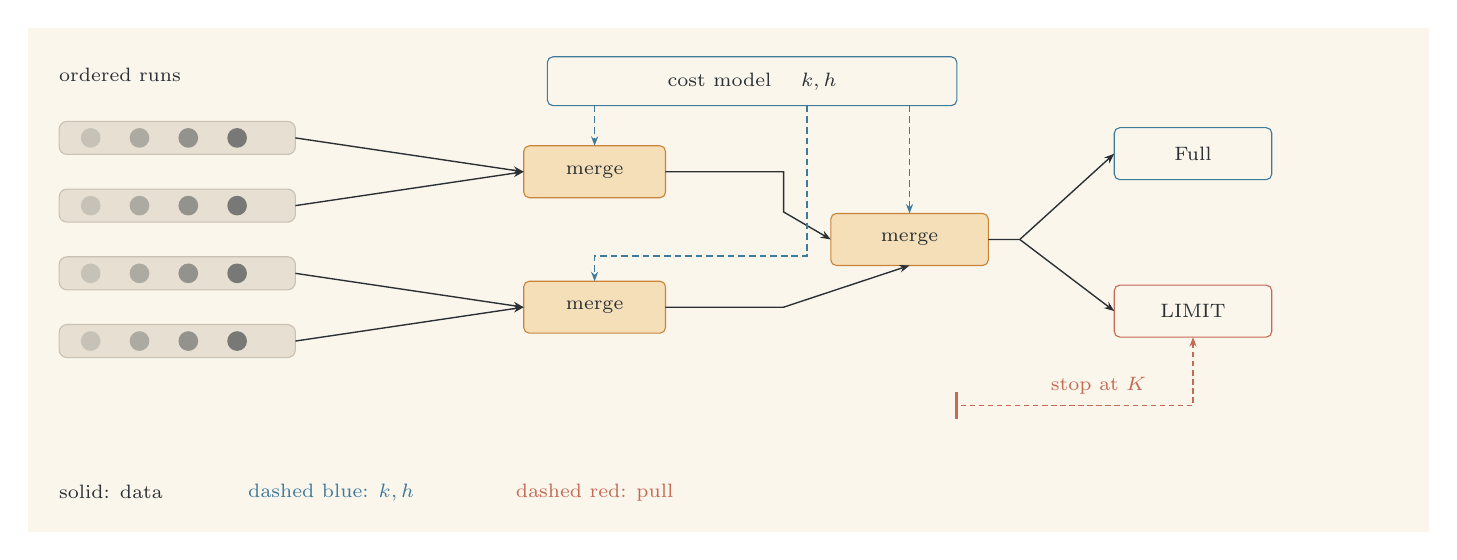
\begin{tikzpicture}[x=1mm,y=1mm,
  every node/.style={inner sep=0pt,outer sep=0pt,text=ink},
  lab/.style={font=\fontsize{7.5}{8.5}\selectfont},
  small/.style={font=\fontsize{6.6}{7.6}\selectfont},
  dat/.style={-{Stealth[length=1.3mm]},draw=ink,line width=0.5pt},
  ctl/.style={-{Stealth[length=1.2mm]},draw=ctrl,line width=0.55pt,dash pattern=on 0.85mm off 0.5mm},
  pull/.style={{Stealth[length=1.2mm]}-,draw=stopc,line width=0.55pt,dash pattern=on 0.7mm off 0.45mm},
  box/.style={draw,rounded corners=0.7mm,minimum height=6.6mm,font=\fontsize{7.5}{8}\selectfont}
]
\useasboundingbox (0,0) rectangle (177.94,64);
\fill[paper] (0,0) rectangle (177.94,64);

% left: ordered runs, anonymous segments
\node[lab,anchor=west] at (4,58) {ordered runs};
\foreach \i in {0,1,2,3} {
  \pgfmathsetmacro{\y}{50-8.6*\i}
  \draw[runedge,rounded corners=1mm,fill=run] (4,\y-2.1) rectangle (34,\y+2.1);
  \foreach \k in {0,1,2,3} {
    \fill[ink,opacity={0.16+0.14*\k}] ({8+6.2*\k},\y) circle (1.25);
  }
}

% merge organization
\node[box,draw=mergeedge,fill=merge,minimum width=18mm] (m1) at (72,45.7) {merge};
\node[box,draw=mergeedge,fill=merge,minimum width=18mm] (m2) at (72,28.5) {merge};
\node[box,draw=mergeedge,fill=merge,minimum width=20mm] (m3) at (112,37.1) {merge};

\draw[dat] (34,50) -- (m1.west);
\draw[dat] (34,41.4) -- (m1.west);
\draw[dat] (34,32.8) -- (m2.west);
\draw[dat] (34,24.2) -- (m2.west);
\draw[dat] (m1.east) -- (96,45.7) -- (96,40.6) -- (m3.west);
\draw[dat] (m2.east) -- (96,28.5) -- (m3.south);

% cost model above the merges; (k,h) drops onto each merge from a free side
\node[draw=ctrl,fill=paper,rounded corners=0.7mm,minimum width=52mm,minimum height=6.2mm,font=\fontsize{7.2}{8.2}\selectfont] (cost) at (92,57.2) {cost model \quad $k,h$};
\draw[ctl] (72,54.1) -- (m1.north);
\draw[ctl] (99,54.1) -- (99,35) -- (72,35) -- (m2.north);
\draw[ctl] (112,54.1) -- (m3.north);

% Full vs LIMIT; short reverse pull stops when K is filled
\node[box,draw=ctrl,minimum width=20mm] (full) at (148,48) {Full};
\node[box,draw=stopc,minimum width=20mm] (lim) at (148,28) {LIMIT};
\draw[dat] (m3.east) -- (126,37.1) -- (full.west);
\draw[dat] (126,37.1) -- (lim.west);
\draw[pull] (lim.south) -- (148,16) -- (118,16);
\draw[stopc,line width=1.15pt] (118,14.3) -- (118,17.7);
\node[small,text=stopc,anchor=south] at (136,17.4) {stop at $K$};

\node[small,anchor=west] at (4,5) {solid: data};
\node[small,text=ctrl,anchor=west] at (28,5) {dashed blue: $k,h$};
\node[small,text=stopc,anchor=west] at (62,5) {dashed red: pull};
\end{tikzpicture}
\end{document}
